% Slides for pp-minbias-13p6tev.

\documentclass[aspectratio=169,11pt]{beamer}

\usetheme{metropolis}
\metroset{progressbar=frametitle, numbering=fraction, sectionpage=progressbar}

\usepackage{cmap}          
\usepackage[T1]{fontenc}
\usepackage{lmodern}
\usepackage{graphicx}
\usepackage{booktabs}
\usepackage{tikz}
\usetikzlibrary{arrows.meta, positioning}

\graphicspath{{../plots/}}

\definecolor{accent}{RGB}{204, 0, 0}
\definecolor{cool}{RGB}{0, 102, 204}
\setbeamercolor{alerted text}{fg=accent}

\newcommand{\pt}{\ensuremath{p_\mathrm{T}}}
\newcommand{\sqs}{\ensuremath{\sqrt{s}}}
\newcommand{\pbar}{\ensuremath{\bar{p}}}
\newcommand{\dndeta}{\ensuremath{\mathrm{d}N_\mathrm{ch}/\mathrm{d}\eta}}

\newcommand{\twoplots}[2]{%
  \begin{center}
    \includegraphics[width=0.48\textwidth]{#1}\hfill
    \includegraphics[width=0.48\textwidth]{#2}
  \end{center}\vspace{-0.6em}}

\newcommand{\twosquares}[3]{%
  \begin{columns}[T]
    \begin{column}{0.35\textwidth}\centering\includegraphics[width=\linewidth]{#1}\end{column}
    \begin{column}{0.35\textwidth}\centering\includegraphics[width=\linewidth]{#2}\end{column}
    \begin{column}{0.27\textwidth}\small #3\end{column}
  \end{columns}}

\newcommand{\fourplots}[4]{%
  \begin{center}
    \includegraphics[width=0.3\textwidth]{#1}\hspace{1em}\includegraphics[width=0.3\textwidth]{#2}\\[-0.2em]
    \includegraphics[width=0.3\textwidth]{#3}\hspace{1em}\includegraphics[width=0.3\textwidth]{#4}
  \end{center}\vspace{-0.6em}}

\title{What happens when two protons collide at $\sqrt{s} = 13.6$\,TeV?}
\subtitle{Minimum-bias pp collisions: Pythia~8 events, a C++/ROOT analysis and a look at ALICE data}
\author{Tomasz Stolarczyk}
\date{November 2026}
\institute{\texttt{github.com/tomekstolarczyk/pp-minbias-13p6tev}}

\begin{document}

\maketitle

% ---------------------------------------------------------------------------------------------
\begin{frame}{Contents}
  \begin{columns}[T]
    \begin{column}{0.5\textwidth}
      \textbf{The task}
      \begin{itemize}
        \item generate $\sim$100\,000 minimum-bias pp collisions at \sqs\ = 13.6\,TeV with Pythia~8
        \item keep only final-state particles
        \item histogram the multiplicity $N$, \pt, $\eta$ and $\phi$ for all charged particles,
              $\pi^\pm$, $K^\pm$, $p$ and \pbar
        \item draw every histogram, export PNG and PDF
      \end{itemize}
    \end{column}
    \begin{column}{0.45\textwidth}
      \textbf{Steps}
      \begin{enumerate}
        \item the setup: generation, analysis, how I read the task
        \item results: the 32 histograms
        \item comparing the categories with each other
        \item comparing the simulation with ALICE data
        \item wrapping up: checks and reproducibility
      \end{enumerate}
    \end{column}
  \end{columns}
\end{frame}

\section{The setup}

% ---------------------------------------------------------------------------------------------
\begin{frame}{The pipeline}
  \centering
  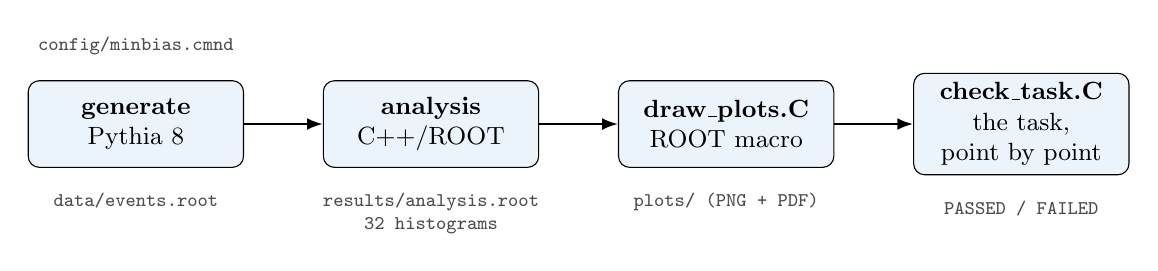
\begin{tikzpicture}[
      box/.style={draw, rounded corners, fill=cool!8, minimum height=1.1cm, text width=2.5cm, align=center, font=\small},
      file/.style={font=\scriptsize\ttfamily, text=black!70},
      arr/.style={-{Latex[length=2mm]}, thick}]
    \node[box] (gen) {\textbf{generate}\\Pythia 8};
    \node[box, right=1.0cm of gen] (ana) {\textbf{analysis}\\C++/ROOT};
    \node[box, right=1.0cm of ana] (draw) {\textbf{draw\_plots.C}\\ROOT macro};
    \node[box, right=1.0cm of draw] (check) {\textbf{check\_task.C}\\the task, point by point};
    \draw[arr] (gen) -- (ana);
    \draw[arr] (ana) -- (draw);
    \draw[arr] (draw) -- (check);
    \node[file, above=0.2cm of gen] {config/minbias.cmnd};
    \node[file, below=0.2cm of gen] {data/events.root};
    \node[file, below=0.2cm of ana, align=center] {results/analysis.root\\32 histograms};
    \node[file, below=0.2cm of draw] {plots/ (PNG + PDF)};
    \node[file, below=0.2cm of check] {PASSED / FAILED};
  \end{tikzpicture}

  \vspace{1.2em}
  \begin{itemize}
    \item \texttt{scripts/run\_all.sh} runs everything with one command, in about 2 minutes (4 with the ALICE comparison)
    \item built with CMake as true C++17; Pythia 8.318, ROOT 6.40.04, GCC 12.3, Ubuntu 22.04
    \item every run leaves its log in \texttt{results/}, so every number in this presentation can be traced back
  \end{itemize}
\end{frame}

% ---------------------------------------------------------------------------------------------
\begin{frame}{Generation}
  \begin{columns}[T]
    \begin{column}{0.48\textwidth}
      \small
      \begin{tabular}{ll}
        \toprule
        \multicolumn{2}{l}{\texttt{config/minbias.cmnd}} \\
        \midrule
        \texttt{Beams:idA, idB}         & 2212, 2212 (pp) \\
        \texttt{Beams:eCM}              & 13600 GeV \\
        \texttt{SoftQCD:inelastic}      & on \\
        \texttt{Tune:pp}                & 14 (Monash 2013) \\
        \texttt{Main:numberOfEvents}    & 100\,000 \\
        \texttt{Random:seed}            & 12345 \\
        \bottomrule
      \end{tabular}
    \end{column}
    \begin{column}{0.48\textwidth}
      \begin{itemize}
        \item only particles with \texttt{isFinal()} are stored: PDG code, charge, \pt, $\eta$, $\phi$
        \item the generator keeps going until exactly 100\,000 good events are stored
        \item 19\,265\,955 final-state particles in total
        \item the settings are also stored inside \texttt{analysis.root}
      \end{itemize}
    \end{column}
  \end{columns}
\end{frame}

% ---------------------------------------------------------------------------------------------
\begin{frame}{Analysis}
  \begin{columns}[T]
    \begin{column}{0.5\textwidth}
      \small
      \begin{tabular}{ll}
        \toprule
        category & selection \\
        \midrule
        \texttt{all}               & every final-state particle \\
        \texttt{ch}                & charge $\neq 0$ \\
        \texttt{pip}, \texttt{pim} & $\pi^+$, $\pi^-$ (PDG $\pm 211$) \\
        \texttt{Kp}, \texttt{Km}   & $K^+$, $K^-$ (PDG $\pm 321$) \\
        \texttt{p}, \texttt{pbar}  & $p$, \pbar\ (PDG $\pm 2212$) \\
        \bottomrule
      \end{tabular}
    \end{column}
    \begin{column}{0.45\textwidth}
      \small
      \begin{tabular}{lll}
        \toprule
        histogram & bins & range \\
        \midrule
        \texttt{hN\_*}   & 400 & $[0, 400]$ \\
        \texttt{hPt\_*}  & 100 & $[0, 10]$ GeV \\
        \texttt{hEta\_*} & 100 & $[-5, 5]$ \\
        \texttt{hPhi\_*} & 64  & $[-\pi, \pi]$ \\
        \bottomrule
      \end{tabular}
    \end{column}
  \end{columns}

  \vspace{1.5em}
  4 quantities $\times$ 8 categories = 32 histograms in \texttt{results/analysis.root}.
  The multiplicity is filled once per event, also when it is zero; \pt, $\eta$ and $\phi$ once per particle.
\end{frame}

% ---------------------------------------------------------------------------------------------
\begin{frame}{How I read the task}
  \small
  \begin{description}[Nothing is thrown away]
    \item[Minimum bias] \texttt{SoftQCD:inelastic}: every inelastic collision, without elastic scattering,
      which makes no new particles. ALICE's own Pythia setup uses the same switch.
    \item[Final state] literally: what \texttt{isFinal()} says, with Pythia's default decays.
    \item[$\phi$ range] the task text gives $[0, \pi]$, Pythia gives $(-\pi, \pi]$; the task author
      confirmed the full range, so \texttt{hPhi} spans $[-\pi, \pi]$ with the 64 bins from the task.
    \item[\texttt{all} and \texttt{ch}] \texttt{all} = every final-state particle, neutral ones included;
      \texttt{ch} = charge $\neq 0$.
    \item[Nothing is thrown away] no cuts; values outside a range go to the under- or overflow bin and
      count in the mean and standard deviation.
  \end{description}
\end{frame}

\section{Results: the 32 histograms}

% ---------------------------------------------------------------------------------------------
\begin{frame}{Results at a glance}
  \centering
  \begin{tabular}{lrrr}
    \toprule
    category & $\langle N\rangle$ per event & $\langle\pt\rangle$ [GeV] & outside $|\eta| < 5$ \\
    \midrule
    all               & 192.66 & 0.40 & 25.7\% \\
    charged           & 92.06  & 0.51 & 26.8\% \\
    $\pi^+$ / $\pi^-$ & 38.36 / 37.71 & 0.48 / 0.48 & 26.1 / 25.0\% \\
    $K^+$ / $K^-$     & 4.24 / 4.12   & 0.68 / 0.68 & 27.7 / 26.0\% \\
    $p$ / \pbar       & 3.82 / 2.60   & 0.69 / 0.78 & 50.3 / 29.0\% \\
    \bottomrule
  \end{tabular}

  \vspace{1em}
  \raggedright
  \begin{itemize}
    \item pions are 83\% of the charged particles, kaons 9\%, protons and antiprotons 7\%
    \item the means include the values outside the histogram ranges
          \hfill{\scriptsize\texttt{results/analysis.log}}
  \end{itemize}
\end{frame}

% ---------------------------------------------------------------------------------------------
\begin{frame}{Multiplicity: all and charged particles}
  \twoplots{histograms_single/hN_all}{histograms_single/hN_ch}
  \small
  \begin{itemize}
    \item 192.7 particles per event, 92.1 of them charged; 12.7\% of the events have $N_\mathrm{all} \geq 400$ and sit in the overflow
    \item $N_\mathrm{ch}$ is always even (the two protons have a total charge of $+2$), so every odd bin of \texttt{hN\_ch} is empty
  \end{itemize}
\end{frame}

\begin{frame}{Multiplicity: $\pi^+$ and $\pi^-$}
  \twoplots{histograms_single/hN_pip}{histograms_single/hN_pim}
  \small
  \begin{itemize}
    \item 38.4 $\pi^+$ and 37.7 $\pi^-$ per event, with a long tail to more than 150
    \item 731 events have no $\pi^+$, 1\,755 have no $\pi^-$
  \end{itemize}
\end{frame}

\begin{frame}{Multiplicity: $K^+$ and $K^-$}
  \twoplots{histograms_single/hN_Kp}{histograms_single/hN_Km}
  \small
  \begin{itemize}
    \item 4.24 $K^+$ and 4.12 $K^-$ per event, about 9 times fewer than pions
    \item 14\,254 events have no $K^+$, 15\,474 have no $K^-$
  \end{itemize}
\end{frame}

\begin{frame}{Multiplicity: $p$ and \pbar}
  \twoplots{histograms_single/hN_p}{histograms_single/hN_pbar}
  \small
  \begin{itemize}
    \item 3.82 protons but only 2.60 antiprotons per event
    \item only \alert{2\,457} events have no proton, against \alert{23\,205} without an antiproton
  \end{itemize}
\end{frame}

% ---------------------------------------------------------------------------------------------
\begin{frame}{Transverse momentum: all and charged particles}
  \twoplots{histograms_single/hPt_all}{histograms_single/hPt_ch}
  \small
  \begin{itemize}
    \item most particles have \pt\ around 0.25 GeV; up to 10 GeV the spectrum falls by about five orders of magnitude
    \item $\langle\pt\rangle$ = 0.40 GeV for all particles, 0.51 GeV for the charged ones: the neutral ones are softer
  \end{itemize}
\end{frame}

\begin{frame}{Transverse momentum: $\pi^+$ and $\pi^-$}
  \twoplots{histograms_single/hPt_pip}{histograms_single/hPt_pim}
  \small
  \begin{itemize}
    \item the two spectra look the same, $\langle\pt\rangle$ = 0.48 GeV for both
    \item 121 $\pi^+$ and 96 $\pi^-$ have $\pt > 10$ GeV and are kept in the overflow
  \end{itemize}
\end{frame}

\begin{frame}{Transverse momentum: $K^+$ and $K^-$}
  \twoplots{histograms_single/hPt_Kp}{histograms_single/hPt_Km}
  \small
  \begin{itemize}
    \item $\langle\pt\rangle$ = 0.68 GeV, higher than for pions; the peak is at 0.35 GeV instead of 0.25 GeV
    \item with fewer particles, the tail above about 5 GeV fluctuates more
  \end{itemize}
\end{frame}

\begin{frame}{Transverse momentum: $p$ and \pbar}
  \twoplots{histograms_single/hPt_p}{histograms_single/hPt_pbar}
  \small
  \begin{itemize}
    \item $\langle\pt\rangle$ = 0.69 GeV for protons, 0.78 GeV for antiprotons
    \item the overlay later shows where the two spectra differ: below about 2 GeV
  \end{itemize}
\end{frame}

% ---------------------------------------------------------------------------------------------
\begin{frame}{Pseudorapidity: all and charged particles}
  \twoplots{histograms_single/hEta_all}{histograms_single/hEta_ch}
  \small
  \begin{itemize}
    \item symmetric around $\eta = 0$, with a shallow dip in the middle
    \item the task range cuts off a lot: 25.7\% of all particles and 26.8\% of the charged ones have $|\eta| > 5$
  \end{itemize}
\end{frame}

\begin{frame}{Pseudorapidity: $\pi^+$ and $\pi^-$}
  \twoplots{histograms_single/hEta_pip}{histograms_single/hEta_pim}
  \small
  \begin{itemize}
    \item a broad plateau with a shallow dip at $\eta = 0$
    \item 26.1\% of the $\pi^+$ and 25.0\% of the $\pi^-$ are outside $|\eta| < 5$
  \end{itemize}
\end{frame}

\begin{frame}{Pseudorapidity: $K^+$ and $K^-$}
  \twoplots{histograms_single/hEta_Kp}{histograms_single/hEta_Km}
  \small
  \begin{itemize}
    \item the dip at $\eta = 0$ is deeper than for pions
    \item 27.7\% of the $K^+$ and 26.0\% of the $K^-$ are outside $|\eta| < 5$
  \end{itemize}
\end{frame}

\begin{frame}{Pseudorapidity: $p$ and \pbar}
  \twoplots{histograms_single/hEta_p}{histograms_single/hEta_pbar}
  \small
  \begin{itemize}
    \item the deepest dip of the three particle types
    \item \alert{50.3\%} of the protons but only 29.0\% of the antiprotons are outside $|\eta| < 5$
  \end{itemize}
\end{frame}

% ---------------------------------------------------------------------------------------------
\begin{frame}{Azimuthal angle: all, charged, $\pi^+$ and $\pi^-$}
  \fourplots{histograms_single/hPhi_all}{histograms_single/hPhi_ch}{histograms_single/hPhi_pip}{histograms_single/hPhi_pim}
  \small
  Flat: mean 0.000 and standard deviation 1.814 = $\pi/\sqrt{3}$, the values of a uniform
  distribution on $[-\pi, \pi]$. No particle falls outside the range.
\end{frame}

\begin{frame}{Azimuthal angle: $K^\pm$, $p$ and \pbar}
  \fourplots{histograms_single/hPhi_Kp}{histograms_single/hPhi_Km}{histograms_single/hPhi_p}{histograms_single/hPhi_pbar}
  \small
  Also flat; with fewer particles per bin, the bin-to-bin fluctuations are larger.
\end{frame}

\section{Comparing the categories}

% ---------------------------------------------------------------------------------------------
\begin{frame}{How to read the overlays}
  \begin{columns}[c]
    \begin{column}{0.4\textwidth}
      \centering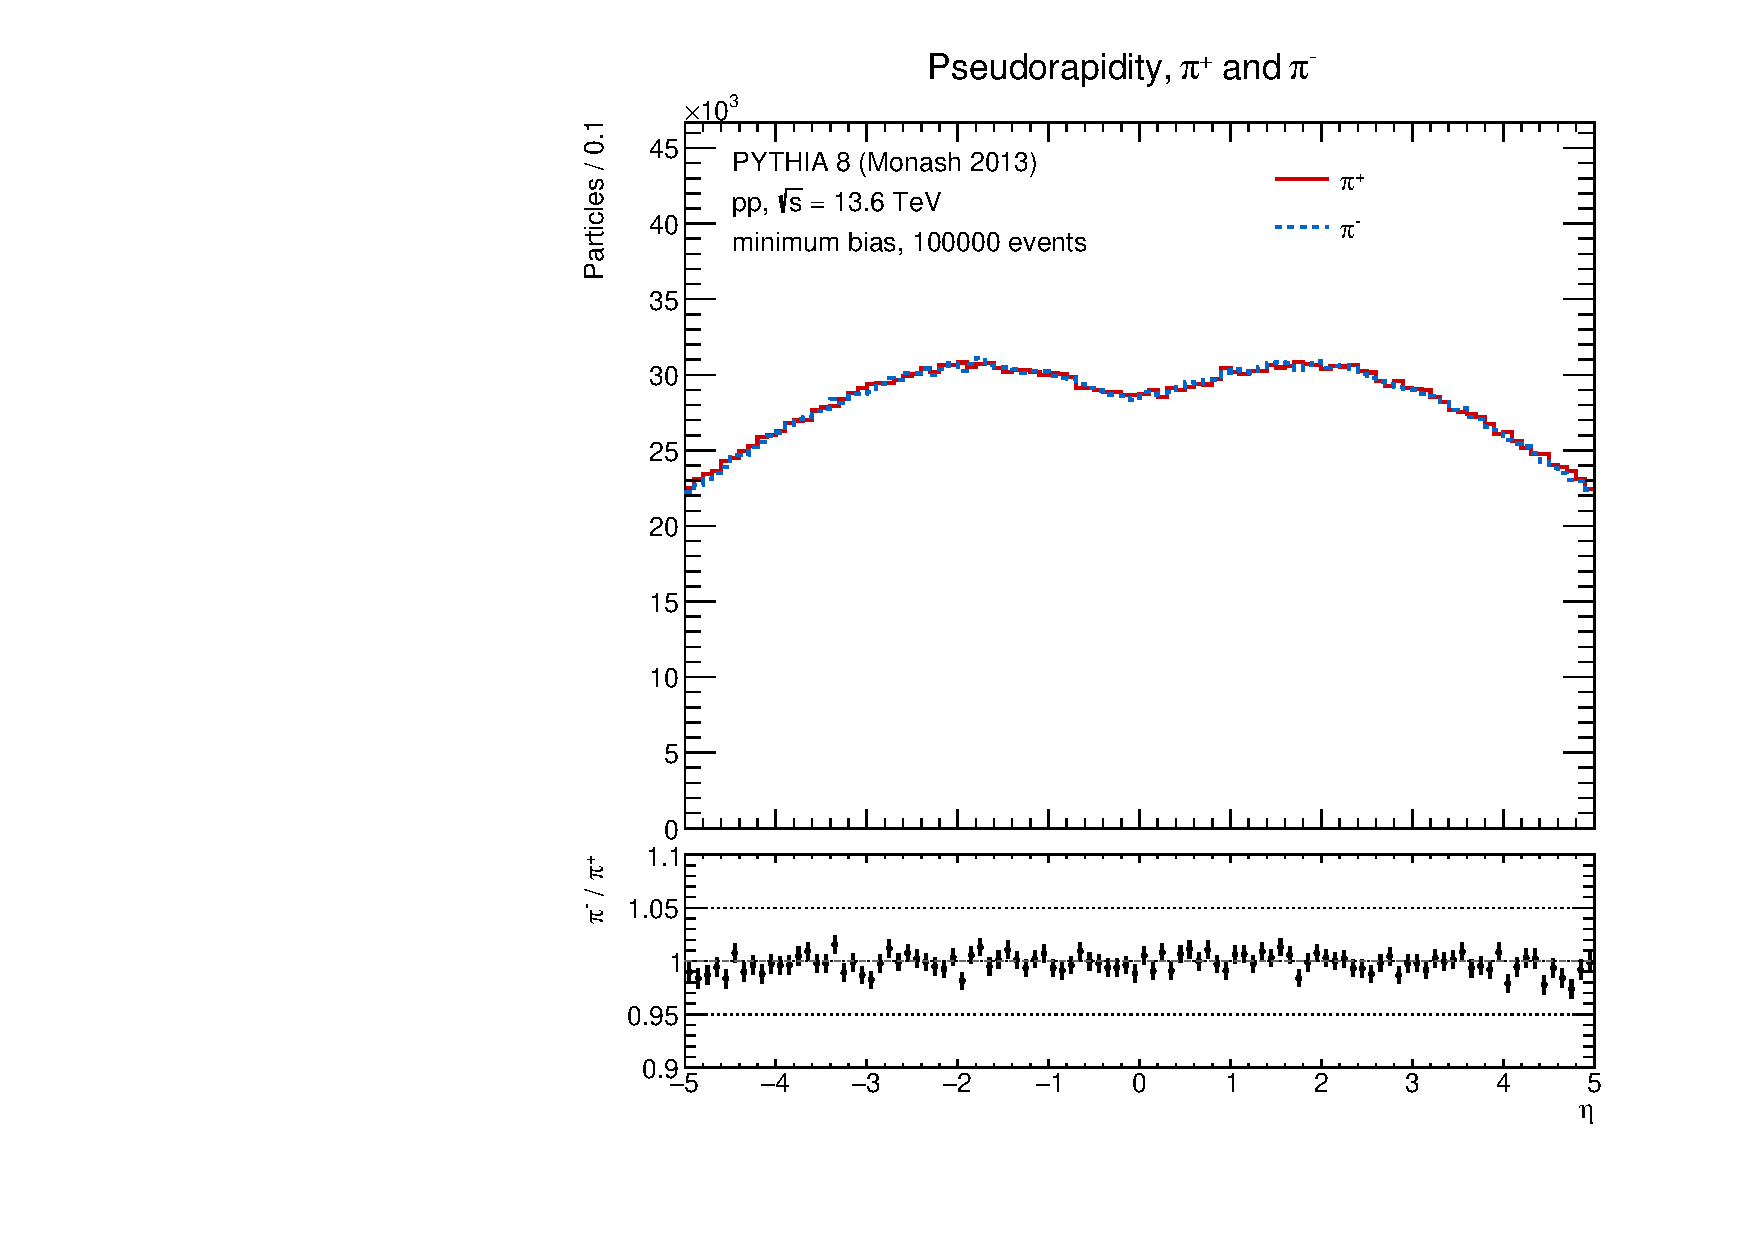
\includegraphics[height=0.8\textheight]{histograms_overlay/eta_pions}
    \end{column}
    \begin{column}{0.56\textwidth}
      \begin{itemize}
        \item two categories on one canvas: {\color{accent}positive} solid, {\color{cool}negative} dashed
        \item the lower panel shows their \alert{ratio}, so differences of a few percent become visible
        \item the error bars come from the bin counts; for charged/all they are binomial,
              because one category is part of the other
        \item where the ratio panel is noisy, there are too few particles to say anything,
              e.g.\ above about 4 GeV for protons
      \end{itemize}
    \end{column}
  \end{columns}
\end{frame}

\begin{frame}{All and charged particles: $N$ and \pt}
  \twosquares{histograms_overlay/multiplicity_all_ch}{histograms_overlay/pt_all_ch}{%
    \begin{itemize}
      \item at the lowest \pt\ only 18\% of the particles are charged; from about 1 GeV on, 69\%
      \item in the event tree, 99\% of the neutral particles below 0.1 GeV are photons
    \end{itemize}}
\end{frame}

\begin{frame}{All and charged particles: $\eta$ and $\phi$}
  \twosquares{histograms_overlay/eta_all_ch}{histograms_overlay/phi_all_ch}{%
    \begin{itemize}
      \item about 47\% of the particles are charged, nearly the same at every $\eta$ (slightly fewer at $\eta = 0$) and every $\phi$
    \end{itemize}}
\end{frame}

\begin{frame}{$\pi^+$ and $\pi^-$: $N$ and \pt}
  \twosquares{histograms_overlay/multiplicity_pions}{histograms_overlay/pt_pions}{%
    \begin{itemize}
      \item the multiplicities almost coincide; at $N = 0$ the $\pi^-$ point is higher
      \item $\pi^-/\pi^+$ is close to 1 at every \pt
    \end{itemize}}
\end{frame}

\begin{frame}{$\pi^+$ and $\pi^-$: $\eta$ and $\phi$}
  \twosquares{histograms_overlay/eta_pions}{histograms_overlay/phi_pions}{%
    \begin{itemize}
      \item $\pi^-/\pi^+ \approx 0.98$, flat in $\eta$ and in $\phi$: a small excess of $\pi^+$ everywhere
    \end{itemize}}
\end{frame}

\begin{frame}{$K^+$ and $K^-$: $N$ and \pt}
  \twosquares{histograms_overlay/multiplicity_kaons}{histograms_overlay/pt_kaons}{%
    \begin{itemize}
      \item $K^-/K^+ \approx 0.97$ at low \pt
      \item above a few GeV the ratio is dominated by statistical fluctuations
    \end{itemize}}
\end{frame}

\begin{frame}{$K^+$ and $K^-$: $\eta$ and $\phi$}
  \twosquares{histograms_overlay/eta_kaons}{histograms_overlay/phi_kaons}{%
    \begin{itemize}
      \item flat ratios, slightly below 1, in $\eta$ and in $\phi$
    \end{itemize}}
\end{frame}

\begin{frame}{$p$ and \pbar: $N$ and \pt}
  \twosquares{histograms_overlay/multiplicity_protons}{histograms_overlay/pt_protons}{%
    \begin{itemize}
      \item \pbar/$p$ rises from \alert{0.55} at the lowest \pt\ to about 0.95 at 2 GeV:
            the extra protons are at low \pt
      \item above about 4 GeV there are too few protons for the ratio to mean anything
    \end{itemize}}
\end{frame}

\begin{frame}{$p$ and \pbar: $\eta$ and $\phi$}
  \twosquares{histograms_overlay/eta_protons}{histograms_overlay/phi_protons}{%
    \begin{itemize}
      \item inside $|\eta| < 5$, \pbar/$p$ = 0.97 and flat
      \item so most of the extra protons are outside the range: 50\% of the protons
            against 29\% of the antiprotons have $|\eta| > 5$
    \end{itemize}}
\end{frame}

% ---------------------------------------------------------------------------------------------
\begin{frame}{Shapes: $\pi$, $K$ and $p$ normalised to unit area}
  \twoplots{histograms_overlay/pt_shapes}{histograms_overlay/eta_shapes}
  \small
  \begin{itemize}
    \item each curve divided by its number of particles, so only the shapes are compared
    \item the mean \pt\ grows with the mass: 0.48, 0.68 and 0.73 GeV for $\pi$, $K$ and $p$+\pbar
    \item the dip at $\eta = 0$ gets deeper with the mass: 93\%, 77\% and 63\% of the maximum
  \end{itemize}
\end{frame}

% ---------------------------------------------------------------------------------------------
\begin{frame}{Two checks hidden in the histograms}
  \begin{columns}[T]
    \begin{column}{0.5\textwidth}
      \textbf{Charge.} Two protons have a total charge of $+2$, so 100\,000 events must have
      200\,000 more positive than negative particles. From the histogram entries:
      \small
      \begin{center}
      \begin{tabular}{lr}
        \toprule
        $\pi^+ - \pi^-$ & 65\,778 \\
        $K^+ - K^-$     & 12\,101 \\
        $p - \pbar$     & 122\,128 \\
        \midrule
        sum             & \alert{200\,007} \\
        \bottomrule
      \end{tabular}
      \end{center}
      The other charged particles ($e$, $\mu$, \dots) make up the remaining $-7$.
    \end{column}
    \begin{column}{0.46\textwidth}
      \textbf{Protons.} The colliding particles are protons, and it shows:
      \begin{itemize}
        \item 3.82 $p$ vs 2.60 \pbar\ per event
        \item 2\,457 events without a proton vs 23\,205 without an antiproton
      \end{itemize}

      \vspace{0.5em}
      A sign mistake in a PDG code would break the charge sum at once, so this is also
      a check of the category selection.
    \end{column}
  \end{columns}
\end{frame}

\section{Comparing with ALICE data}

% ---------------------------------------------------------------------------------------------
\begin{frame}{Finding a paper to compare with}
  A simulation is a model, and a model is only as good as its agreement with real data.

  \vspace{0.5em}
  arXiv, ALICE papers with 13.6\,TeV in the title:
  \small
  \begin{itemize}
    \item D$^{*+}$-meson spin alignment (2609.39713)
    \item B$^0$-meson production cross section (2603.18904)
    \item time resolution of the TOF detector (2511.10311)
    \item \alert{Inclusive and multiplicity-dependent pseudorapidity densities of charged particles} (2602.10658)
  \end{itemize}
  \normalsize
  Only the last one is about the same particles: the $\eta$ distribution of charged particles,
  per event and per unit of $\eta$ (\dndeta). That is my \texttt{hEta\_ch}, divided by the number
  of events and the bin width.
\end{frame}

\begin{frame}{Counting the way ALICE counts}
  \begin{columns}[T]
    \begin{column}{0.5\textwidth}
      \textbf{Events:} the paper reports \alert{INEL$>$0} collisions, with at least one charged
      particle in $|\eta| < 1$. I apply the same selection.

      \vspace{0.8em}
      \textbf{Decays:} ALICE's own Pythia configuration (AliceO2, \texttt{pythia8\_inel.cfg}) lets only
      particles with $c\tau_0 < 10$ mm decay, so $K^0_S$, $\Lambda$ and similar particles stay undecayed.
      My comparison run does the same (\texttt{config/minbias\_alice.cmnd}).
    \end{column}
    \begin{column}{0.45\textwidth}
      \small
      Effect of the decay setting, per event:
      \begin{center}
      \begin{tabular}{lrr}
        \toprule
                  & default & ALICE \\
        \midrule
        charged   & 92.06 & 83.77 \\
        $\pi^+$   & 38.36 & 34.45 \\
        $K^+$     & 4.24  & 4.24 \\
        $p$       & 3.82  & 3.05 \\
        \bottomrule
      \end{tabular}
      \end{center}
      $\pi^+$ $-10\%$, $p$ $-20\%$, kaons unchanged.
    \end{column}
  \end{columns}
\end{frame}

\begin{frame}{One definition at a time}
  \begin{columns}[c]
    \begin{column}{0.55\textwidth}
      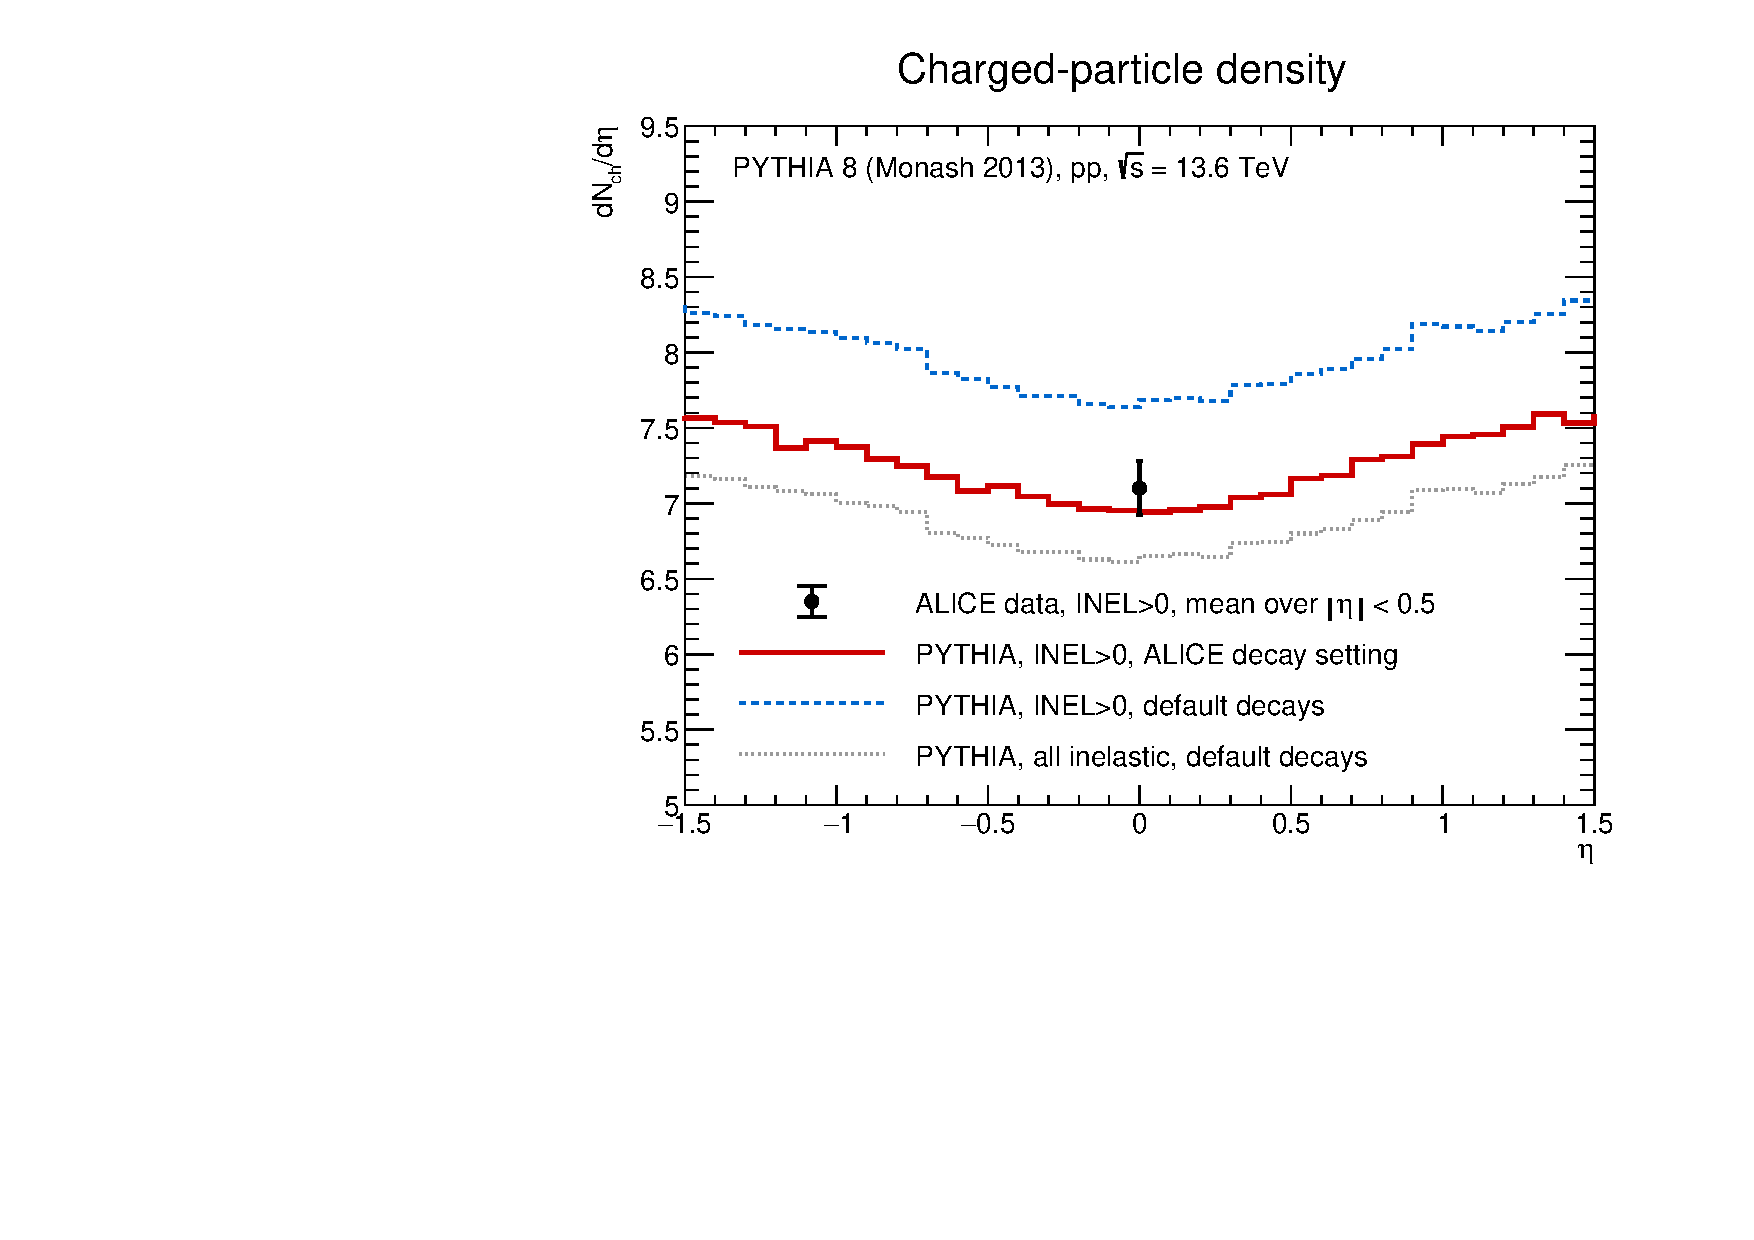
\includegraphics[width=\textwidth]{alice_comparison/alice_fig1_dndeta}
    \end{column}
    \begin{column}{0.43\textwidth}
      \small
      $\langle\dndeta\rangle$ in $|\eta| < 0.5$:

      \begin{tabular}{lr}
        \toprule
        task run                 & 6.675 \\
        + only INEL$>$0          & 7.713 \\
        + ALICE decay setting    & \alert{7.004} \\
        \midrule
        ALICE measurement        & \alert{7.10 $\pm$ 0.18} \\
        \bottomrule
      \end{tabular}

      \vspace{0.5em}
      With the same definitions, PYTHIA agrees with the measurement within its uncertainty
      (ratio 0.987).
    \end{column}
  \end{columns}
\end{frame}

\begin{frame}{Multiplicity classes}
  \begin{columns}[T]
    \begin{column}{0.56\textwidth}
      \footnotesize
      \begin{tabular}{lrrrr}
        \toprule
        class (\%) & data & \shortstack[r]{PYTHIA\\(ALICE)} & \shortstack[r]{PYTHIA\\(mine)} & \shortstack[r]{mine/\\data} \\
        \midrule
        0--1    & 21.78 $\pm$ 0.38 & 25.50 & 25.96 & 1.19 \\
        1--5    & 18.48 $\pm$ 0.25 & 20.71 & 20.91 & 1.13 \\
        5--10   & 15.76 $\pm$ 0.22 & 17.19 & 17.44 & 1.11 \\
        10--15  & 13.89 $\pm$ 0.19 & 14.71 & 14.66 & 1.06 \\
        15--20  & 12.50 $\pm$ 0.17 & 12.62 & 12.58 & 1.01 \\
        20--30  & 10.86 $\pm$ 0.15 & 10.02 & 10.10 & 0.93 \\
        30--40  & 9.09 $\pm$ 0.13  & 7.51  & 7.60  & 0.84 \\
        40--50  & 7.63 $\pm$ 0.11  & 5.60  & 5.64  & 0.74 \\
        50--70  & 5.87 $\pm$ 0.09  & 3.72  & 3.76  & 0.64 \\
        70--100 & 3.69 $\pm$ 0.06  & 2.47  & 2.49  & 0.68 \\
        \midrule
        0--100  & 7.10 $\pm$ 0.18  & 7.11  & 7.00  & 0.99 \\
        \bottomrule
      \end{tabular}

      \vspace{0.2em}
      {\scriptsize $\langle\dndeta\rangle$ in $|\eta| < 0.5$, INEL$>$0; classes as in Table 2 of the paper}
    \end{column}
    \begin{column}{0.4\textwidth}
      \small
      ALICE sorts the collisions by the signal in its forward detector FT0 (Table 2 of the paper).
      I count charged particles in the same $\eta$ ranges and split my events the same way.
      \begin{itemize}
        \item my PYTHIA matches theirs within 2\% in every class
        \item the average agrees, the extremes do not: 19\% too many particles in the busiest class,
              up to 36\% too few in the quiet ones, as the paper also reports
      \end{itemize}
    \end{column}
  \end{columns}
\end{frame}

\section{Wrapping up}

% ---------------------------------------------------------------------------------------------
\begin{frame}{The task, checked point by point}
  \small
  \texttt{tests/check\_task.C} runs at the end of every pipeline run:
  \begin{center}
  \begin{tabular}{lp{0.62\textwidth}}
    \toprule
    task & what is checked \\
    \midrule
    technical  & build with \texttt{-std=c++17}, ROOT 6, Pythia 8 \\
    1) generation & pp, \texttt{Beams:eCM = 13600}, SoftQCD, 100\,000 events, total charge $+2$ in every event \\
    2), 3) histograms & 32 names, binning and ranges, one \texttt{hN} entry per event, every $\phi$ in $[-\pi, \pi]$,
                        each category holds exactly its particles \\
    4) macro & opens \texttt{analysis.root}, axis labels, legends, every plot as PNG and PDF \\
    \bottomrule
  \end{tabular}
  \end{center}
  Each check was tested by breaking its line of code on purpose (wrong PDG sign, no \texttt{isFinal()},
  $N = 0$ not filled, wrong number of bins) and watching it fail.
\end{frame}

\begin{frame}{Reproducible by design}
  \begin{itemize}
    \item one command, \texttt{scripts/run\_all.sh}: build, generate, analyse, draw, check, compare
    \item the random seed is fixed in the \texttt{.cmnd} file, and the Pythia settings are stored
          inside \texttt{analysis.root} in a form Pythia can read back
    \item checked on a fresh clone from GitHub: \texttt{run\_all.sh} in 3 min 46 s, every task check passed,
          all 32 histograms \alert{bin-for-bin identical} to the committed ones
    \item every log is in the repository: Pythia's settings and error statistics, every histogram's mean,
          standard deviation and out-of-range counts, the ALICE comparison
  \end{itemize}
\end{frame}

\begin{frame}{Summary}
  \begin{itemize}
    \item $N_\mathrm{ch}$ is always even, and there are more $\pi^+$, $K^+$ and $p$ than $\pi^-$, $K^-$ and \pbar
    \item the extra protons are at low \pt\ and mostly outside $|\eta| < 5$
    \item heavier particles have a higher mean \pt\ and a deeper dip at $\eta = 0$
    \item with ALICE's definitions, PYTHIA matches the measured average density at 13.6 TeV,
          but not the busiest and the quietest collisions
    \item every step runs with one command, is checked against the task and gives the same histograms every time
  \end{itemize}
\end{frame}

\begin{frame}[standout]
  Thank you!

  \vspace{1em}
  \normalsize
  \texttt{github.com/tomekstolarczyk/pp-minbias-13p6tev}

  \vspace{0.5em}
  \footnotesize
  ALICE has not published identified-particle spectra at 13.6 TeV yet.\\
  I hope that changes soon, and I would be glad to help :)
\end{frame}

\end{document}
